\documentclass[border=2pt]{standalone}
% Figura dell'architettura (compilata a parte: TikZ e' in conflitto con ieeeaccess.cls)
\usepackage{mathptmx}
\usepackage{amsmath,bm}
\usepackage{tikz}
\usetikzlibrary{positioning,arrows.meta}
\begin{document}
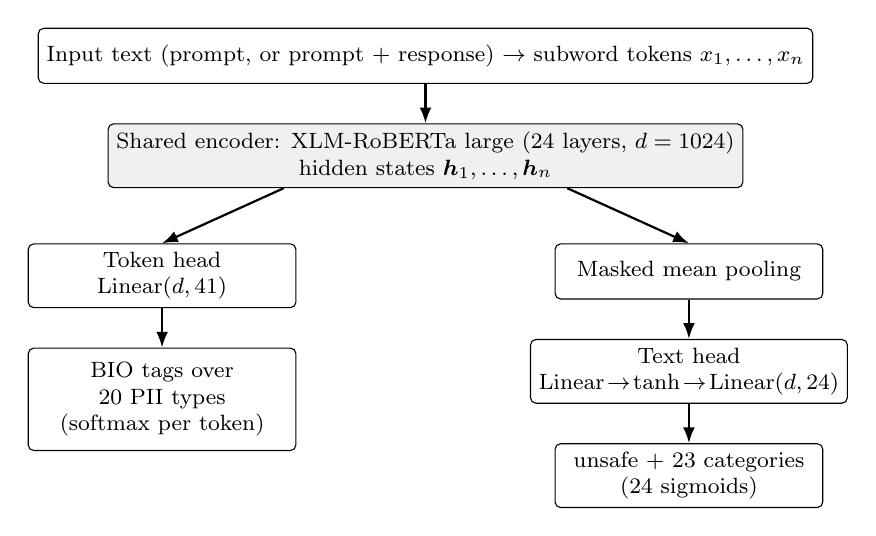
\begin{tikzpicture}[
  font=\footnotesize, node distance=5mm and 4mm,
  box/.style={draw, rounded corners=2pt, align=center, minimum height=7mm, inner sep=3pt},
  arr/.style={-{Latex[length=2mm]}, thick}]
\node[box, minimum width=7.6cm] (in) {Input text (prompt, or prompt + response) $\rightarrow$ subword tokens $x_1,\dots,x_n$};
\node[box, fill=gray!12, minimum width=7.6cm, below=of in] (enc) {Shared encoder: XLM-RoBERTa large (24 layers, $d=1024$)\\ hidden states $\bm{h}_1,\dots,\bm{h}_n$};
\node[box, below left=7mm and -24mm of enc, minimum width=3.4cm] (ph) {Token head\\ $\mathrm{Linear}(d, 41)$};
\node[box, below right=7mm and -24mm of enc, minimum width=3.4cm] (pool) {Masked mean pooling};
\node[box, below=of pool, minimum width=3.4cm] (sh) {Text head\\ $\mathrm{Linear}\!\rightarrow\!\tanh\!\rightarrow\!\mathrm{Linear}(d, 24)$};
\node[box, below=of ph, minimum width=3.4cm, minimum height=13mm] (po) {BIO tags over\\ 20 PII types\\ (softmax per token)};
\node[box, below=of sh, minimum width=3.4cm] (so) {unsafe + 23 categories\\ (24 sigmoids)};
\draw[arr] (in) -- (enc);
\draw[arr] (enc.south) ++(-1.8cm,0) -- (ph.north);
\draw[arr] (enc.south) ++(1.8cm,0) -- (pool.north);
\draw[arr] (pool) -- (sh);
\draw[arr] (ph) -- (po);
\draw[arr] (sh) -- (so);
\end{tikzpicture}
\end{document}
